%!TEX program = xelatex

\documentclass[usepdftitle=false]{beamer}

% Good bibliography
\RequirePackage[backend=biber]{biblatex}
\addbibresource[datatype=bibtex]{biblio.bib}

\RequirePackage{hyperref}

\hypersetup{
	pdftitle			= {Sarek, an introduction},
	pdfsubject		= {Sarek - introduction},
	pdfkeywords		= {Somatic, Germline, Variations, Cancer, Workflow, Container, Reproducibility, Nextflow, Pipeline, Singularity, Docker, Genomics, Exome},
	pdfauthor			= {Maxime U. Garcia},
	pdfcreator		= {\LaTeX},
	pdfproducer		= {XeTeX 3.14159265-2.6-0.99996}}

% Icon Fonts
\RequirePackage{academicons}
\RequirePackage{fontawesome}

% Correct the path when including svg pictures
\RequirePackage{import}

% For nice verbatim
\RequirePackage{minted}
\definecolor{LightGray}{HTML}{D3D3D3}
\setmintedinline{bgcolor=LightGray}

% To resize graphic and table
\RequirePackage{graphics}

% For captions
\RequirePackage{caption}

% Arrange theme
\usetheme[
	progressbar=frametitle,
	sectionpage=none,
	numbering=fraction
]{metropolis}

\makeatletter
	\setlength{\metropolis@titleseparator@linewidth}{1pt}
	\setlength{\metropolis@progressonsectionpage@linewidth}{2pt}
	\setlength{\metropolis@progressinheadfoot@linewidth}{2pt}
\makeatother

% Color the progress:
% - SciLifeLabGreen (#7FCB28) for SciLifeLab
% - KIplum for KI (#8C0058)
\definecolor{SciLifeLabGreen}{HTML}{7FCB28}
\definecolor{KIplum}{HTML}{8C0058}
\setbeamercolor{progress bar}{fg=SciLifeLabGreen,bg=white}
\setbeamercolor{progress bar in head/foot}{fg=KIplum,bg=white}

\newcommand{\ts}{\textsuperscript}

\title{%
	\vspace{-1.2cm}%
	
\includegraphics[height=1cm]{pictures/Sarek_no_border_white}%
}

\subtitle{%
	\normalsize{An introduction}%
	\vspace{-.4cm}%
}

\titlegraphic{
	\hspace{4.9cm}
\includegraphics[height=.9cm]{pictures/SciLifeLab-white}%
	\hfill
\includegraphics[height=.9cm]{pictures/KI-horizontal-white}%
	\vspace{.3cm}%

	\hspace{4.9cm}
\includegraphics[height=.7cm]{pictures/NGI-white}%
	\hfill
\includegraphics[height=.7cm]{pictures/NBIS-green}%
	\vspace{.5cm}%

	\hspace{4cm}\hfill\includegraphics[height=1.2cm]{pictures/Barntumörbanken-white}%
}

\author{
	\vspace{-.6cm}
	\faUser\ Maxime U. Garcia\\
	\faGlobe\ \href{https://maxulysse.github.io/}{maxulysse.github.io}\\
	\faGithub\ \href{https://github.com/MaxUlysse/}{@MaxUlysse}\\
	\faTwitter\ \href{https://twitter.com/gau/}{@gau}\\
}

\date{\vfill}

\begin{document}

\section{Sarek}

{
	\usebackgroundtemplate{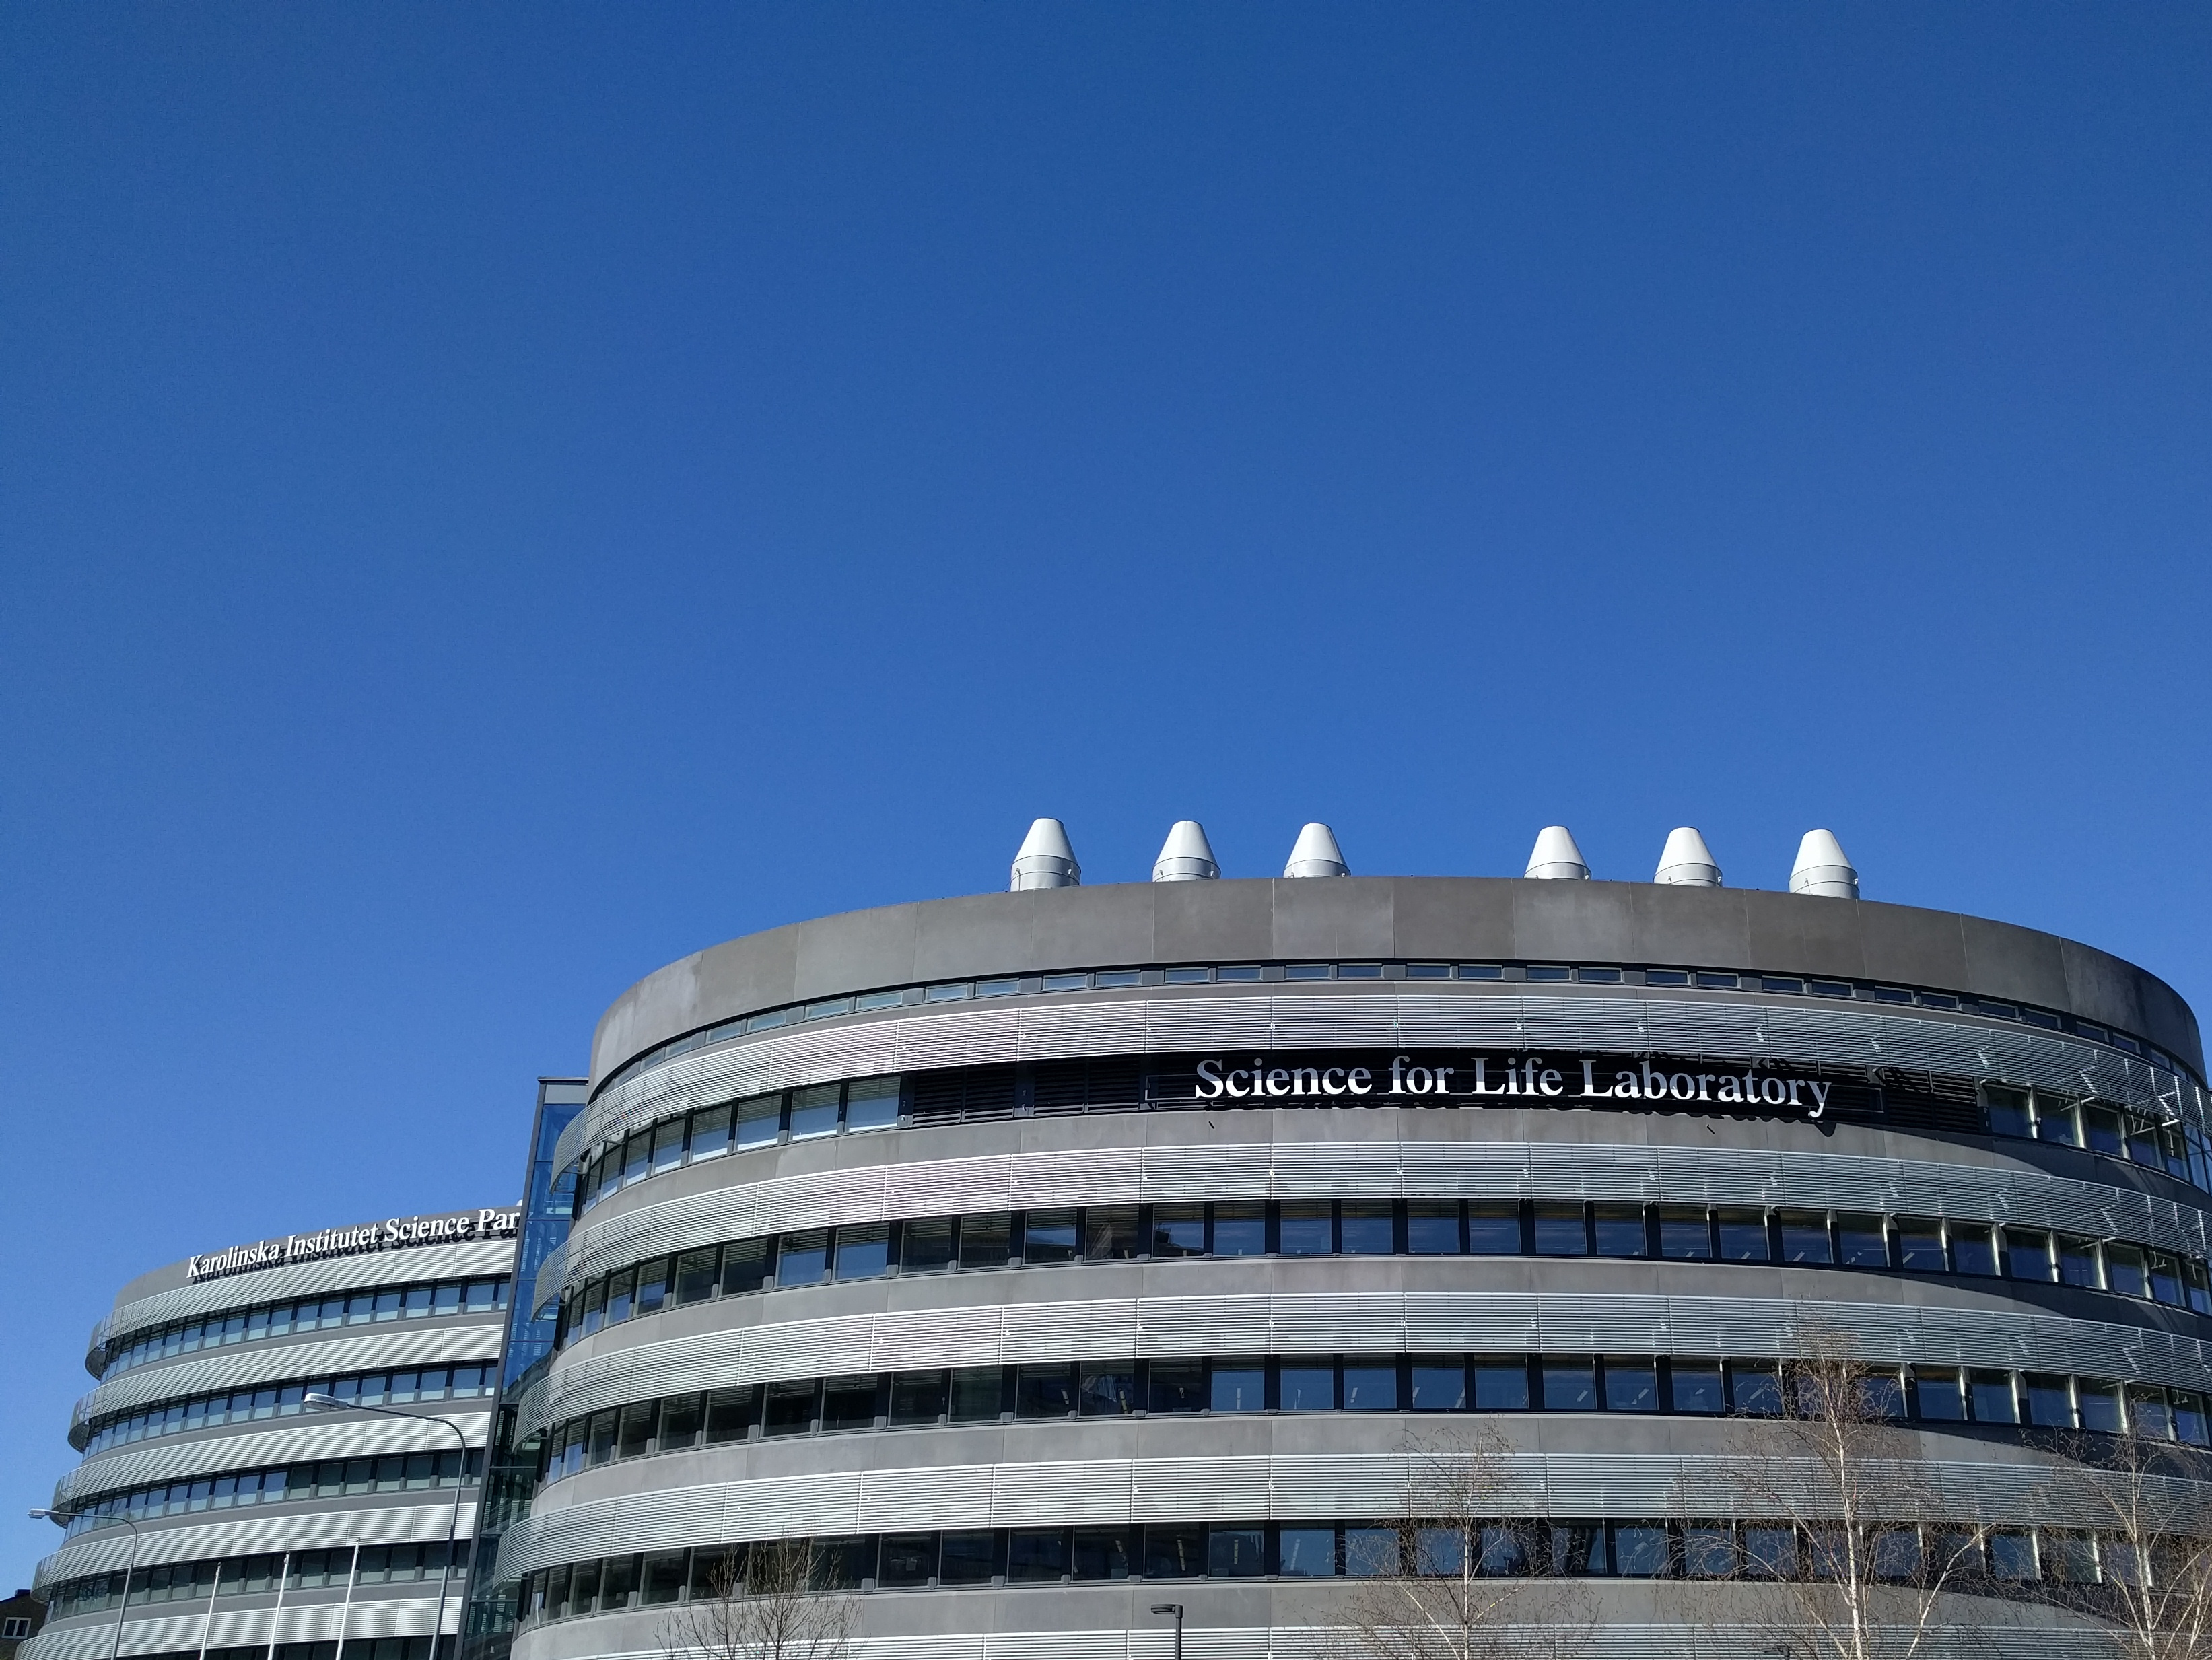
\includegraphics[width=\paperwidth]{pictures/SciLifelab-BlueSky2.jpg}}
	\setbeamercolor{normal text}{fg = white, bg = white}
	\maketitle
}

\section{Data types}

\begin{frame}{Samples}
	\begin{figure}
		
\includegraphics[height=2.5cm]{pictures/Samples}
	\end{figure}
	\begin{itemize}
		\item Normal sample -> blood
		\pause
		\item Tumor sample
		\pause
		\item Eventual relapse or metastasis
	\end{itemize}
\end{frame}

\begin{frame}{WGS - WES - Targeted sequencing}
	\begin{figure}
		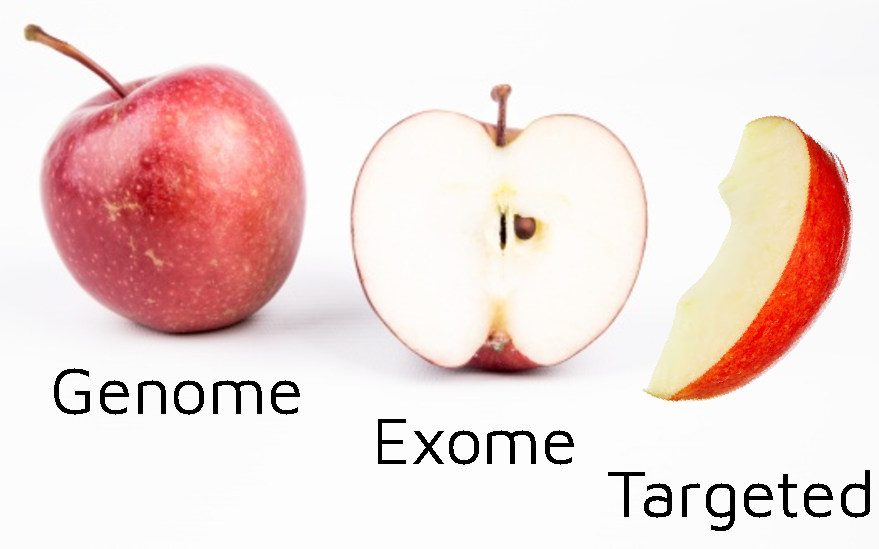
\includegraphics[height=5cm]{pictures/AppleSeq}
	\end{figure}
\end{frame}

\begin{frame}{Sequencing}
	\begin{figure}
		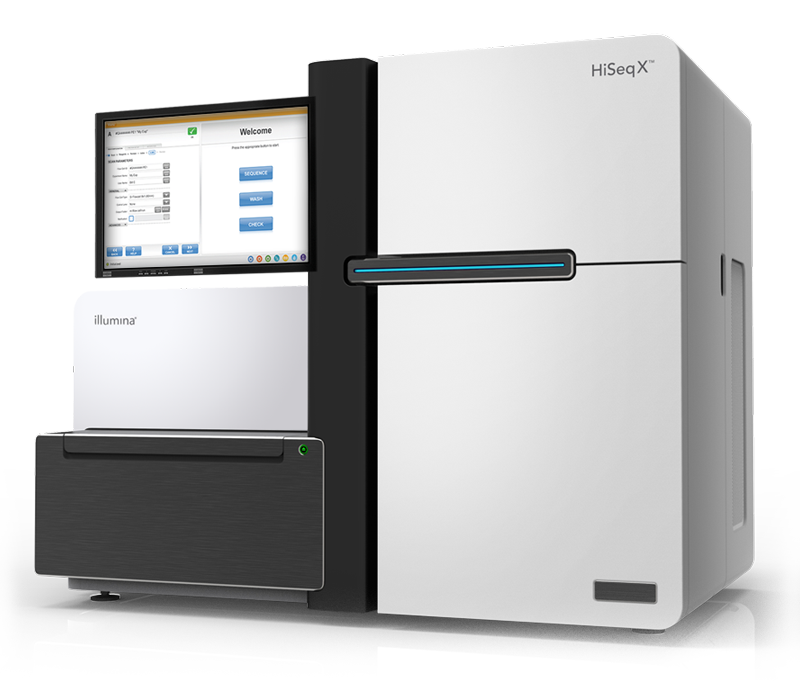
\includegraphics[height=4cm]{pictures/hiseq-x.png}
		\captionof*{figure}{Illumina's HiSeq X}
	\end{figure}
	\begin{itemize}
		\item Short reads
	\end{itemize}
\end{frame}

\begin{frame}[fragile]{FASTQ Files}
	FASTQ: text-based format for storing both nucleotide sequence and corresponding quality scores.
	\pause

	\begin{itemize}
		\item At least 1 for each samples (single end)
		\pause
		\item At least 1 pair for each samples (pair end)
	\end{itemize}

	\pause
	\begin{minted}[fontsize=\scriptsize]{text}
  @SEQ_ID
  GATTTGGGGTTCAAAGCAGTATCGATCAAATAGTAAATCCATTTGTTCAACTCACAGTTT
  +
  !''*((((***+))%%%++)(%%%%).1***-+*''))**55CCF>>>>>>CCCCCCC65
	\end{minted}

\end{frame}

\begin{frame}{Preprocessing}
	\begin{itemize}
		\item Map short reads to reference genome
		\pause
		\item Cleanup
	\end{itemize}
\end{frame}

\begin{frame}[fragile]{SAM/BAM files}
	Sequence Alignment Map (SAM): text-based format for storing biological sequences aligned to a reference sequence.
	\pause

	Binary Alignment Map (BAM): compressed binary representation of SAM format.
	\pause

	\begin{minted}[fontsize=\scriptsize]{text}
  @HD VN:1.6 SO:coordinate
  @SQ SN:ref LN:45
  r001 99 ref 7 30 8M2I4M1D3M = 37 39 TTAGATAAAGGATACTG *
  r002 0 ref 9 30 3S6M1P1I4M * 0 0 AAAAGATAAGGATA *
  r003 0 ref 9 30 5S6M * 0 0 GCCTAAGCTAA * SA:Z:ref,29,-,6H5M,17,0;
  r004 0 ref 16 30 6M14N5M * 0 0 ATAGCTTCAGC *
  r003 2064 ref 29 17 6H5M * 0 0 TAGGC * SA:Z:ref,9,+,5S6M,30,1;
  r001 147 ref 37 30 9M = 7 -39 CAGCGGCAT * NM:i:1
	\end{minted}
\end{frame}

\begin{frame}{Variant Calling}
	\begin{itemize}
		\item Germline
		\pause
		\begin{itemize}
			\item Differences to Reference genome
		\end{itemize}
		\pause
		\item Somatic
		\pause
		\begin{itemize}
			\item Differences to Germline genome
		\end{itemize}
	\end{itemize}
\end{frame}

\begin{frame}[fragile]{VCF files}
	The Variant Call Format (VCF): text-based format for storing gene sequence variations.
	\pause

	\begin{minted}[fontsize=\scriptsize]{text}
  ##fileformat=VCFv4.3
  ##fileDate=20090805
  ##source=myImputationProgramV3.1
  ##reference=file:///seq/references/1000GenomesPilot-NCBI36.fasta
  ##phasing=partial
  #CHROM POS ID REF ALT QUAL FILTER INFO FORMAT NA00001 NA00002 NA00003
  20 14370 rs6054257 G A 29 PASS NS=3;DP=14;AF=0.5;DB;H2 GT:GQ:DP:HQ
    0|0:48:1:51,51 1|0:48:8:51,51 1/1:43:5:.,.
  20 17330 . T A 3 q10 NS=3;DP=11;AF=0.017 GT:GQ:DP:HQ
    0|0:49:3:58,50 0|1:3:5:65,3 0/0:41:3
  20 1110696 rs6040355 A G,T 67 PASS NS=2;DP=10;AF=0.333,0.667;AA=T;DB GT:GQ:DP:HQ
    1|2:21:6:23,27 2|1:2:0:18,2 2/2:35:4
  20 1230237 . T . 47 PASS NS=3;DP=13;AA=T GT:GQ:DP:HQ
    0|0:54:7:56,60 0|0:48:4:51,51 0/0:61:2
  20 1234567 microsat1 GTC G,GTCT 50 PASS NS=3;DP=9;AA=G GT:GQ:DP
    0/1:35:4 0/2:17:2 1/1:40:3
	\end{minted}
\end{frame}

\begin{frame}{What do we want?}
	\begin{figure}
		
\includegraphics[height=2cm]{pictures/doanalysis}
	\end{figure}
	\pause
	\begin{itemize}
		\item Easy to use
		\pause
		\item Easy to install
		\pause
		\item Reproducible
		\pause
		\item Portable
		\pause
		\item Open Source
		\pause
		\item QC
	\end{itemize}
\end{frame}

\begin{frame}{What do we need?}
	\begin{itemize}
		\item Tools
		\pause
		\begin{itemize}
			\item Installation
			\item Version
		\end{itemize}
		\pause
		\item Reference files
		\pause
		\begin{itemize}
			\item Dowload
			\item Version
		\end{itemize}
		\pause
		\item Annotation files
		\pause
		\begin{itemize}
			\item Dowload
			\item Version
		\end{itemize}
		\pause
		\item Works with cluster executor
	\end{itemize}
\end{frame}

\section{Sarek}

\begin{frame}{What is Sarek?}
	\begin{figure}
		
\includegraphics[height=1.5cm]{pictures/Sarek_no_border}
		\captionof*{figure}{\faGlobe\ \url{http://sarek.scilifelab.se/}}
	\end{figure}
	\begin{itemize}
		\item Analysis germline and somatic workflow
		\item<2-> Whole genome or targeted sequencing
		\item<3-> Developed with NGI and NBIS
		\item<4-> Support from The Swedish Childhood Tumor Biobank
	\end{itemize}
	\begin{figure}
		
\includegraphics[height=.8cm]{pictures/blank}<-2>
		
\includegraphics[height=.8cm]{pictures/NGI}<3->
		\only<4->{\hfill}
		\includegraphics[height=.8cm]{pictures/Barntumörbanken}<4->
		\only<3->{\hfill}
		
\includegraphics[height=.8cm]{pictures/NBIS-orange}<3->
	\end{figure}
	\vfill
\end{frame}

\section{What's inside}

\begin{frame}{Nextflow}
	\begin{figure}
		
\includegraphics[height=1.5cm]{pictures/nextflow.png}
		\captionof*{figure}{\faGlobe\ \url{https://www.nextflow.io/}}
	\end{figure}
	\begin{itemize}
		\item Data-driven workflow language
		\pause
		\item Portable (executable on multiple platforms)
		\pause
		\item Shareable and reproducible (with containers)
	\end{itemize}
	\vfill
\end{frame}

\begin{frame}{Singularity}
	\begin{figure}
		
\includegraphics[height=2cm]{pictures/Singularity}
		\captionof*{figure}{\faGlobe\ \url{https://www.sylabs.io/singularity/}}
	\end{figure}
	\begin{itemize}
		\item Docker-like container engine
		\begin{itemize}
			\item Specific for HPC environnment
		\end{itemize}
		\pause
		\item Without the root user security problem
		\pause
		\item Supported by Nextflow
		\pause
		\item Can pull containers from Docker-hub
	\end{itemize}
\end{frame}

\begin{frame}{Sarek exists in multiple flavors}
	\begin{figure}
		
\includegraphics[height=1.5cm]{pictures/Sarek}
	\end{figure}
	\vfill
	\pause
	\begin{center}
		
\includegraphics[height=1.5cm]{pictures/Sarek_germline}
		\hfill
		\pause
		
\includegraphics[height=1.5cm]{pictures/Sarek_somatic}
	\end{center}
	\pause
	\begin{center}
		
\includegraphics[height=1.5cm]{pictures/Sarek_exome}
	\end{center}
\end{frame}

\begin{frame}{Data and files workflow}
	\begin{figure}
		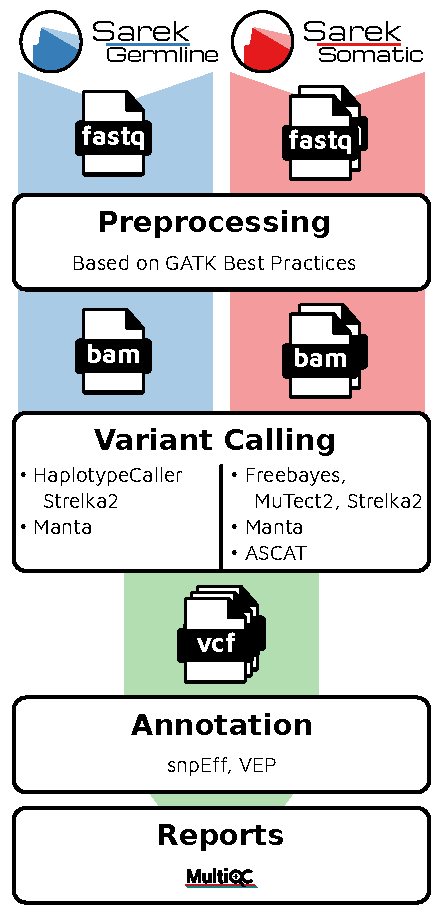
\includegraphics[height=7cm]{pictures/Sarek_2-2_workflow}
	\end{figure}
\end{frame}

\begin{frame}{Preprocessing}
	\begin{figure}
		
\includegraphics[height=1cm]{pictures/GATKBP}
		\captionof*{figure}{\faGlobe\ \url{https://software.broadinstitute.org/gatk/best-practices/}}
	\end{figure}
	Based on GATK Best Practices (GATK 4.0)
	\pause

	\begin{itemize}
		\item Reads mapped to reference genome with \mintinline{text}{bwa}
		\pause
		\item Duplicates marked with \mintinline{text}{picard MarkDuplicates}
		\pause
		\item Recalibrate with \mintinline{text}{GATK BaseRecalibrator}
	\end{itemize}

\end{frame}

\begin{frame}{Germline Variant Calling}
	\begin{itemize}
		\item SNVs and small indels:
		\pause
	\begin{itemize}
			\item HaplotypeCaller
			\item Strelka2
		\end{itemize}
		\pause
		\item Structural variants:
		\pause
		\begin{itemize}
			\item Manta
		\end{itemize}
	\end{itemize}
\end{frame}

\begin{frame}{Somatic Variant Calling}
	\begin{itemize}
		\item SNVs and small indels:
		\pause
		\begin{itemize}
			\item MuTect2
			\item Freebayes
			\item Strelka2
		\end{itemize}
		\pause
		\item Structural variants:
		\pause
		\begin{itemize}
			\item Manta
		\end{itemize}
		\pause
		\item Sample heterogeneity, ploidy and CNVs:
		\pause
		\begin{itemize}
			\item ASCAT
			\item Control-FREEC (\faWrench\ adding)
		\end{itemize}
	\end{itemize}
\end{frame}

\begin{frame}{Annotation}
	\begin{itemize}
		\item VEP and SnpEff
		\item \faDatabase\ ClinVar, COSMIC, dbSNP, GENCODE, gnomAD, polyphen, sift, etc.
	\end{itemize}
\end{frame}


\begin{frame}{\faWrench\ Prioritization}
	\begin{itemize}
		\item	First step towards clinical use
		\pause
		\item	Rank scores are computed for all variants
		\begin{itemize}
			\item	COSMIC, ClinVar, SweFreq and MSK-IMPACT (cancerhotspots.org)
		\end{itemize}
		\pause
		\item	Findings are ranked in three tiers
		\begin{itemize}
			\item	1\ts{st} tier: well known, high-impact variants
			\item	2\ts{nd} tier: variants in known cancer-related genes
			\item	3\ts{rd} tier: the remaining variants
		\end{itemize}
	\end{itemize}
\end{frame}

\section{Acknowledgments}

\begin{frame}{Acknowledgments}
	\begin{figure}
		
\includegraphics[height=.6cm]{pictures/Barncancerfonden}%
		\hfill%
		
\includegraphics[height=.6cm]{pictures/KI-horizontal}%
		\hfill%
		\includegraphics[height=.6cm]{pictures/Barntumörbanken}%
		\hfill%
		
\includegraphics[height=.6cm]{pictures/SciLifeLab}%
	\end{figure}
	\begin{table}
		\resizebox{\textwidth}{!}{%
		\begin{tabular}{llllll}
		\textbf{Barntumörbanken}	&	Elisa Basmaci								&	\textbf{NGI}	&	Johannes Alneberg						&	\textbf{NBIS}	&	Sebastian DiLorenzo	\\
															&	Szilveszter Juhos						&								&	Anandashankar Anil					&								&	Malin Larsson	\\
															&	Gustaf Ljungman							&								&	Franziska Bonath						&								&	Marcel Martin	\\
															&	Monica Nistèr								&								&	Orlando Contreras‐López			&								&	Markus Mayrhofer	\\
															&	Gabriela Prochazka					&								&	Phil Ewels									&								&	Björn Nystedt	\\
															&	Johanna Sandgren						&								&	Sofia Haglund								&								&	Markus Ringnér	\\
															&	Teresita Díaz De Ståhl			&								&	Max Käller									&								&	Pall I Olason	\\
															&	Katarzyna Zielinska-Chomej	&								&	Anna Konrad									&								&	Jonas Söderberg	\\
															&															&								&	Pär Lundin									&								&	\\
		\textbf{Grupp Nistèr}	&	Saad Alqahtani			&														&	Remi-Andre Olsen						&	\textbf{Clinical Genomics}	&	Kenny Billiau\\
													&	Min Guo							&														&	Senthilkumar Panneerselvam	&															&	Hassan Foroughi Asl\\
													&	Daniel Hägerstrand	&														&	Fanny Taborsak							&															&	Valtteri Wirta\\
													&	Anna Hedrén					&														&	Chuan Wang									&															&	\\
													&	Martin Proks				&									&							&	\textbf{Nextflow folks}	&	Paolo Di Tommaso	\\
													&	Rong Yu							&									&							&													&	Sven Fillinger	\\
													&	Jian Zhao						&	\textbf{Clinical Genetics}		&	Jesper Eisfeldt			&		&	Alexander Peltzer	\\
		\end{tabular}}
	\end{table}
	\begin{figure}
		
\includegraphics[height=.5cm]{pictures/NGI}%
		\hfill%
		
\includegraphics[height=.5cm]{pictures/NBIS-orange}%
		\hfill%
		
\includegraphics[height=.5cm]{pictures/nextflow.png}%
		\hfill%
		
\includegraphics[height=.5cm]{pictures/nf-core}%
		\hfill%
		
\includegraphics[height=.5cm]{pictures/uppmax.png}%
	\end{figure}
\end{frame}

{
	\usebackgroundtemplate{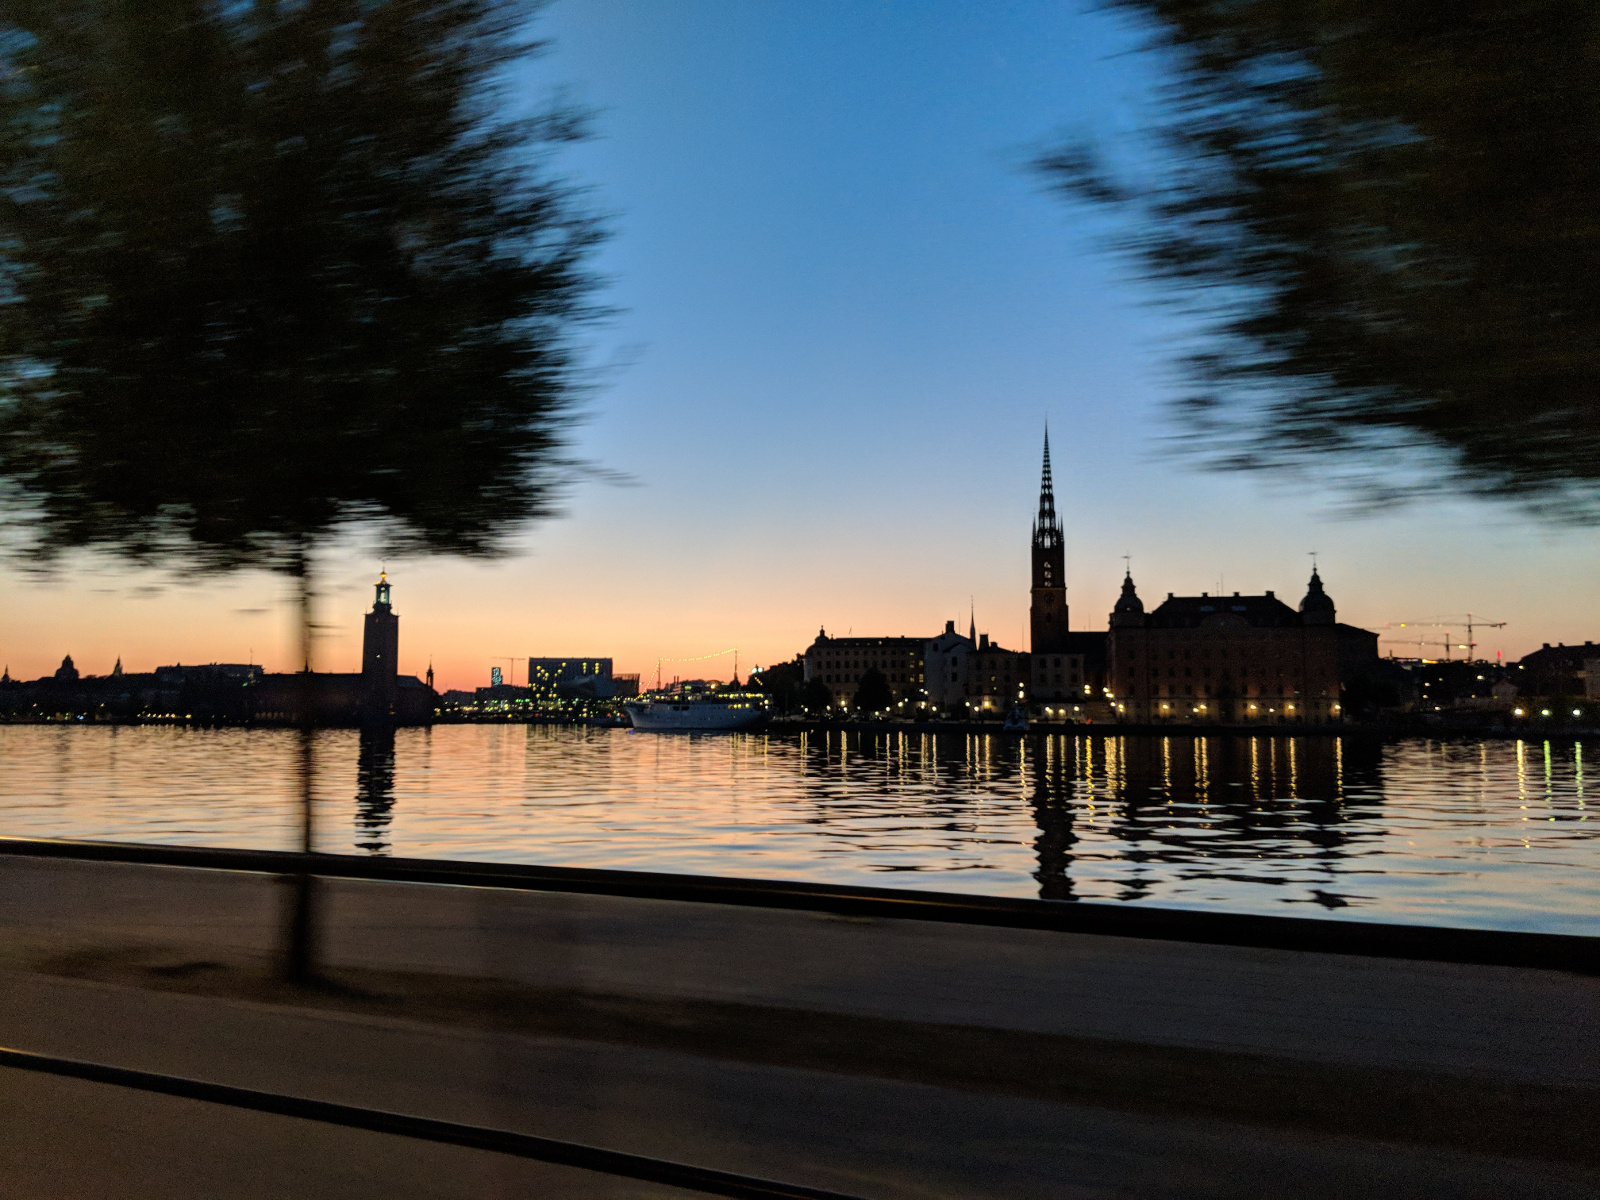
\includegraphics[height=\paperheight]{pictures/Stockholm-by-night.jpg}}
	\setbeamercolor{normal text}{fg = white}
	\setbeamercolor{frametitle}{fg = white, bg = black!80}
	\usebeamercolor[fg]{normal text}
	\section{Questions}
	\begin{frame}[plain]{Any questions?}
	\vspace{-6cm}
	\faGlobe\ \url{http://sarek.scilifelab.se/}

	\faGithub\ \url{https://github.com/SciLifeLab/Sarek}
	\end{frame}
}

\end{document}
